\scanpage{19}
% L1–2
Son déterminant est égal à
\[
0!\;1!\;2!\;\unsure{\text{\textemdash}|\ldots|\cdots}\;(p-1)!
\]
% L3–6
qui provient donc d'un élément non nul de $\mathbb Z/pZ$, donc est inversible dans $C$, i.e. les $D^i$ $(0\leq i\leq p-1)$ forment bien une base de $\operatorname{Hom}_{\unsure{,|A}}(C,C)$ sur $C$. Donc

% L7–11
\uline{Proposition} Soit $C$ une $A$-algèbre ayant une
\par\noindent\begin{tabular}{|p{.92\linewidth}}
$p$-base réduite à un élément. Alors $C$ est\inserted{\unsure{?}} un espace homogène fibré principal sous $\unsure{\mathcal U|U}=A[X]/X^pA[X]$ (\deleted{\unsure{de}}de la façon explicitée plus haut)
\end{tabular}

% L12, section divider
\figure{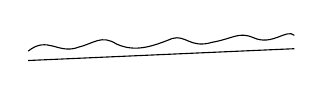
\begin{tikzpicture}[x=1cm,y=1cm]
\draw (0,0) .. controls (.25,.20) and (.38,-.05) .. (.64,.05)
 .. controls (.84,.10) and (.93,.21) .. (1.12,.09)
 .. controls (1.36,-.02) and (1.58,.06) .. (1.83,.16)
 .. controls (2.00,.21) and (2.06,.03) .. (2.33,.11)
 .. controls (2.61,.16) and (2.67,.25) .. (2.86,.17)
 .. controls (3.10,.06) and (3.28,.29) .. (3.38,.20);
\draw (0,-.12)--(3.38,.03);
\end{tikzpicture}}
% L13–16
\uuline{Questions} 1) Soit $C$ comme plus haut. Déterminer \unsure{ttes} les façons possibles de \deleted{\unsure{réduire la|réduire le} \unsure{rang}} \inserted{\unsure{'obtenir|définir} \unsure{la|C}} $C$-hyperalgèbre \deleted{Hom} tordue $\operatorname{Hom}_A(C,C)$ à partir d'une sous-$A$-hyperalgèbre $U$
% L17–21
(libre de rang $p$ sur $A$). Déterminer les $U$ \deleted{pour lesquels} qui sont isomorphes à l'algèbre enveloppante restreinte d'une $p$-algèbre de Lie \inserted{sur $A$, qui est un module} libre de rang 1\,; d'une \inserted{telle} $p$-algèbre \deleted{qui} avec puissance $p^{\text{ième}}$ nulle
% archive sheet number: 18
